%template1.tex
%The following LaTeX source file represents the simplest kind of slide presentation; no overlays, no included graphics. Substitute your favorite style for ``pascal''. To create the PDF file template1.pdf, (1) be sure to use the prosper class, then (2) execute the command latex template1.tex, and (3) the command dvipdf template1.dvi.

%%%%%%%%%%%%%%%%%%%%%%%%%%%%%%% template1.tex %%%%%%%%%%%%%%%%%%%%%%%%%%%%%%%%%%%
\documentclass[a4paper,blends,pdf,colorBG,slideColor]{prosper}
% definitions for slides for CSC544
% Lutz Hamel, (c) 2007

\hypersetup{pdfpagemode=FullScreen}

\usepackage{amssymb}
\usepackage{latexsym}
\usepackage{amsmath}
%\usepackage[usenames]{color}
\usepackage{xypic}


\newcommand{\term}[1]{\ensuremath{\mbox{\bf #1}}}
\newcommand{\nonterm}[1]{\ensuremath{\mbox{#1}}}
\newcommand{\ifstmt}[3]{\ensuremath{{\bf if}\; {#1}\;{\bf then}\;{#2}\;{\bf else}\;{#3}\;\term{end}}}
\newcommand{\whilestmt}[2]{\ensuremath{{\bf while}\; {#1}\;{\bf do}\;{#2}\; \term{end}}}
\newcommand{\funcstmt}[3]{\ensuremath{{\bf fun}\; {#1}\; {\bf is}\; {#2} \; {\bf return}\; {#3}}}
\newcommand{\syntaxset}[1]{\ensuremath{\mbox{\bf #1}}}
\newcommand{\orbar}{\;|\;}
\newcommand{\bs}[1]{\begin{slide}{#1}\ptsize{8}}
\newcommand{\es}{\end{slide}}
\newcommand{\co}{\,\colon\;}
\newcommand{\pair}[2]{\ensuremath{\langle {#1}, {#2} \rangle}}
\newcommand{\encode}[1]{\ensuremath{\langle {#1} \rangle}}
\newcommand{\mytab}{\makebox[.15in]{}}
%\newcommand{\abs}[1]{{\mid{#1}\mid}}
\newcommand{\abs}[1]{{|{#1}|}}
\newcommand{\ol}[1]{\overline{#1}}

\newcommand{\qaccept}{\ensuremath{q_{\mbox{\tiny accept}}}}
\newcommand{\qreject}{\ensuremath{q_{\mbox{\tiny reject}}}}
\newcommand{\accept}{{\em accept}}
\newcommand{\reject}{{\em reject}}

\newcommand{\machine}[1]{
	\begin{quote}
	{#1}
	\end{quote}
	}

\newcommand{\fdef}[1]{
	\begin{center}
	\fbox{
	\begin{minipage}{3.5in}
	{\bf Definition:}
	{#1}
	\end{minipage}
	}
	\end{center}
	}

\newcommand{\ftheorem}[1]{
	\begin{center}
	\fbox{
	\begin{minipage}{3.5in}
	{\bf Theorem:}
	{#1}
	\end{minipage}
	}
	\end{center}
	}

\newcommand{\flemma}[1]{
	\begin{center}
	\fbox{
	\begin{minipage}{3.5in}
	{\bf Lemma:}
	{#1}
	\end{minipage}
	}
	\end{center}
	}


\newcommand{\fframe}[1]{
	\begin{center}
	\fbox{
	\begin{minipage}{3.5in}
	{#1}
	\end{minipage}
	}
	\end{center}
	}

\newcommand{\nframe}[1]{
	\begin{center}
	\begin{minipage}{3.5in}
	{#1}
	\end{minipage}
	\end{center}
	}

\begin{document}
\bs{Strings \& Languages}
Sequences or strings of symbols and characters are fundamental in computer science.
We use strings of symbols to represent data and most importantly we use them to
represent algorithms.

We formalize these structures as follows:

An {\bf alphabet} is any non-empty, finite set. The elements of an alphabet are called {\bf symbols}.

{\bf Examples:}
\[
\Sigma = \{ 0, 1\}
\]
\[
\Sigma' = \{ a, b, c, d \}
\]
\[
\Gamma = \{ this, and, that \}
\]

A {\bf string over an alphabet} is a finite sequence of symbols from that alphabet.

{\bf Example:} Given the alphabet $\Sigma = \{0, 1\}$ then the following are
strings over this alphabet: $011001$, $000000$, $1$.
\es

\bs{Operations on Strings}
If $w$ is a string over $\Sigma$, then the {\bf length} of $w$, written $|w|$, is
the number of symbols  $w$ contains.

The {\bf empty string}, usually written as $\epsilon$, is a string where $|\epsilon|=0$.

Given a string $w$ of length $n$, we can write $w = w_1  w_2\ldots w_n$ where
$w_i \in \Sigma$. Furthermore, we can define the {\bf reverse} of $w$ by
 $w^R = w_n w_{n-1}\ldots w_1$.
 
 Some string $z$ is a {\bf substring} of $w$ if $z$ appears consecutively within $w$,
 e.g., $cd$ is a substring of $abcdef$.
 
 Given two strings $x = x_1 x_2\ldots x_n$ and $y = y_1 y_2\ldots y_m$ where
 $x_i, y_j \in \Sigma$ for $i = 1\ldots n$ and $j = 1 \ldots m$, then the
 {\bf concatenation} of $x$ and $y$ is obtained by appending $y$ to the
 end of $x$ written as $xy = x_1 x_2 \ldots x_n y_1 y_2 \ldots y_m$ with $|xy| = n + m$.
 
 Given a string that consists of $k$ copies of the same symbol, we use a superscript
 notation for compactness,
 \[
\overbrace{xx\ldots x}^k = x^k.
\]

\es

\bs{Languages}
\vspace{.9in}
\begin{center}
\fbox{
\LARGE \em {\bf Definition:} A {\bf language} is a set of strings.
}
\end{center}

\es

\bs{Languages}
{\bf Example:} The language $L_2$ of all 2 bit words. Let $\Sigma = \{0,1\}$ be
the alphabet, then we can construct strings such as $01$, $0001$, {\em etc.}. But
our language is only the set of all 2 bit words, thus
\[
L_2 = \{ 00, 01, 10, 11 \}.
\]

{\bf Example:} The language $L_a$ consisting of words of five or less $a$'s.  
Let $\Sigma = \{a\}$ be the alphabet, then we construct strings such as $a$, $aaa$,
then our language is
\[
L_a = \{ a, aa, aaa, aaaa, aaaaa\}.
\]

{\bf Note:} The empty language is not equivalent to the language that has the
empty string as its only member,
\[
L_\emptyset = \{ \} \not\equiv L_\epsilon = \{ \epsilon \}.
\]
\es

\bs{Course Road Map}
\begin{center}
    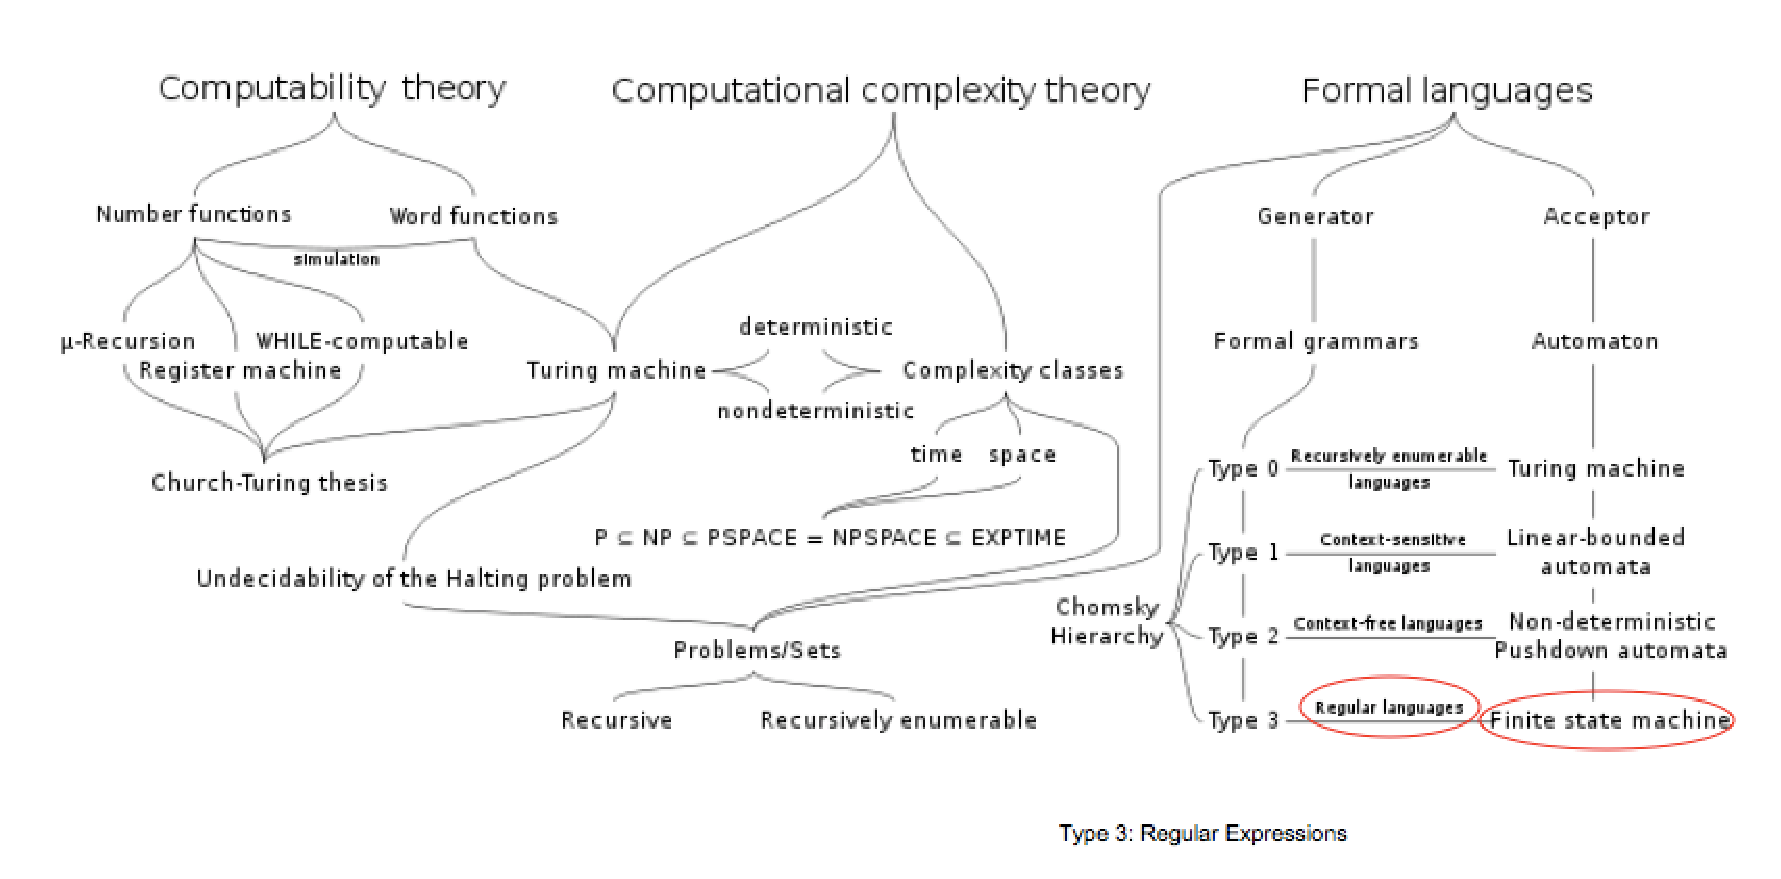
\includegraphics[height=45mm]{images/course-road-map-02.eps}
\end{center}

\es

\bs{Regular Languages}
\begin{itemize}
\item The simplest model of computation we know is the {\bf finite automaton}.
\item As we will see, this machine computes via {\bf state transitions} given {\bf input strings}.
\item We say that a computation is successful if a FA {\bf accepts} a particular string.
\item If all the strings of a particular language are accepted then we say that the FA {\bf recognizes} that language.
\end{itemize}

In the following we formally define these notions. 

\es

\bs{FA - Example}
\begin{center}
    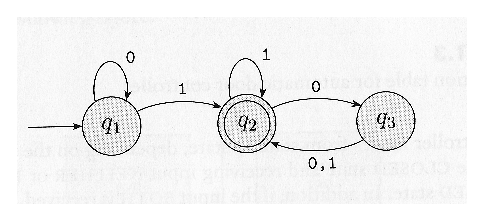
\includegraphics[height=35mm]{images/FA-01.eps}
\end{center}

\vspace{.2in}
Terms: states, start state, accept states, state transitions, alphabet.

Which of the strings would the above machine accept: $000$, $01$, $010$?

What would a machine look like for $L_2$ and $L_a$, respectively?
\es

\bs{Formal Def. of FA}
Pictures are nice but they are not very useful when we try to develop a mathematical
theory of computing.  We need a more formal definition:
\vspace{.5in}

{\bf Definition:} a {\bf finite automaton} is a 5-tuple $(Q, \Sigma, \delta, q_0, F)$, where
\begin{enumerate}
\item $Q$ is a finite set called the {\bf states},
\item $\Sigma$ is a finite set called the {\bf alphabet},
\item $\delta\co Q \times \Sigma \rightarrow Q$ is the {\bf transition function},
\item $q_0 \in Q$ is the {\bf start state}, and
\item $F \subseteq Q$ is the {\bf set of accept states}.
\end{enumerate}

\es

\bs{FA - Example, again}
\begin{center}
    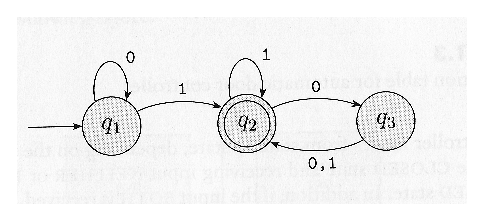
\includegraphics[height=15mm]{images/FA-01.eps}
\end{center}
{\small
\begin{enumerate}
\item $Q =\{q_1, q_2, q_3\}$,
\item $\Sigma = \{0,1\}$,
\item $\delta\co Q \times \Sigma \rightarrow Q$ can be described by a table,

\begin{tabular}{c | c c}
& $0$ & $1$\\ \hline
$q_1$ & $q_1$ & $q_2$\\
$q_2$ & $q_3$ & $q_2$\\
$q_3$ & $q_2$ & $q_2$
\end{tabular}

\item $q_1 \in Q$ is the {\bf start state}, and
\item $F = \{q_2\}$.
\end{enumerate}
}
\es

\bs{Language of a Machine}
Let $M$ be some FA and $A$ be the set of all strings that the machine accepts, then we 
say that $A$ is the {\bf language of machine $M$} or, alternatively, that
{\bf $M$ recognizes $A$} and we write
\[
L(M) = A.
\]

{\bf Example:} Let $M_1$ be our machine
\begin{center}
    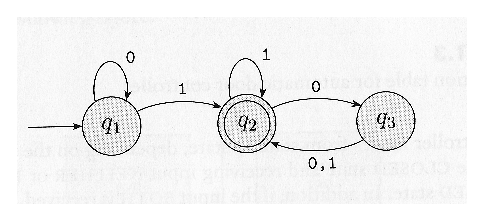
\includegraphics[height=15mm]{images/FA-01.eps}
\end{center}
we can determine that this machine accepts all the strings in the set
\[
B = \{ w \mid \mbox{$w$ contains at least one $1$ followed by a combination of $1$, $00$, or $01$}\},
\]
then we say that $L(M_1) = B$ or $M_1$ recognizes $B$.
\es

\bs{Formal Def. of Computation}
Let $M = (Q, \Sigma, \delta, q_0, F)$ be a FA and let $w = w_1 w_2 \ldots w_n$
be a string  with $w_i \in \Sigma$, then $M$ {\bf accepts} $w$
if a sequence of states $q_0, q_1, \ldots, q_n$ with $q_i \in Q$ exists with conditions:
\begin{enumerate}
\item $\delta(q_i, w_{i+1}) = q_{i+1}$, for $i = 0, \ldots, n-1$, and
\item $q_n \in F$.
\end{enumerate}

Sometimes we write
\[
q_0 w_1 w_2 \ldots w_n \vdash  w_1 q_1 w_2 \ldots w_n \vdash  \ldots  \vdash 
 w_1 w_2 \ldots q_{n-1}w_n \vdash  w_1 w_2 \ldots w_n q_n
\]
for the computation.\footnote{Here the symbol $\vdash$ means `entails'.}

We say that $M$ {\bf recognizes language} $A$ if $A = \{w \mid M \mbox{ accepts } w\}$.

\vspace{.3in}

\framebox{{\bf Definition:} A language is called a {\bf regular language} if some finite
automaton recognizes it}
\es
\end{document}
%%%%%%%%%%%%%%%%%%%%%%%%%%% end of template1.tex %%%%%%%%%%%%%%%%%%%%%%%%%%%%%%%%

